\chapter{Adaptive Control System} \label{ch:acs}

Adaptive controller is generally referred to a controller with adjustable parameters and associated mechanism to adjust such parameters, to conform to new circumstances.

Comparing with most of the other control systems, an adaptive control system does not require a very precise modeling of the plant. More precisely, an adaptive control system can adapt the control gains to the unknown or time-varying plant and maintain the stability of the closed-loop system.

The references of this chapter include:
\begin{itemize}
	\item Åström, K.J. and Wittenmark, B., 2013. Adaptive control. Courier Corporation \cite{aastrom2013adaptive}.
\end{itemize}

\section{Introduction}

Adaptive controller is generally referred to a controller with adjustable parameters and associated mechanism to adjust such parameters, to conform to new circumstances.

Due to the parameter adjustment mechanism, the controller becomes non-linear. For example, while a conventional PID controller is linear, an adaptive PID controller is nonlinear since the $P(t)$, $I(t)$ and $D(t)$ are variables instead of constant gains.

In practice, an adaptive controller is often a modified version of a conventional controller just like the adaptive PID controller example. There are often 2 types of feedback loops in an adaptive control system: the original loops that comes with the conventional controller, and the additional loops to adjust the parameters of the conventional controller. A demonstrative figure is given in Fig. \ref{ch:acs:fig:adaptive_control_schema_general}.

\begin{figure}
	\centering
	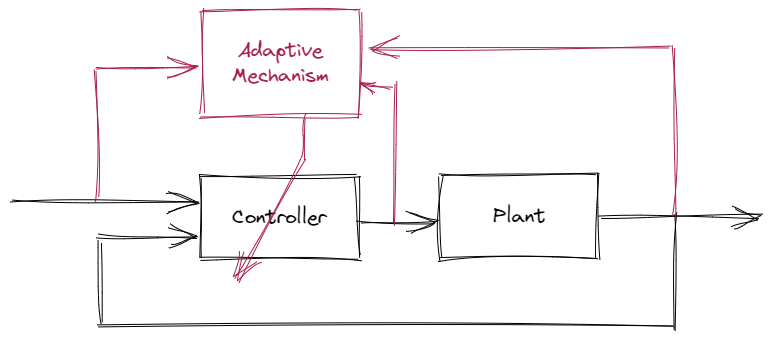
\includegraphics[width=300pt]{chapters/ch-adaptive-control-system/figures/adaptive_control_schema_general.png}
	\caption{Adaptive control system general schema.} \label{ch:acs:fig:adaptive_control_schema_general}
\end{figure}

\subsection{A Brief History of Adaptive Control System}

The first adaptive control system application was designed for autopilots of a high-performance aircraft, where the conventional control system was found to work for one condition but not for the other. Gain scheduling was adopted to solve this problem.

Later on more sophisticated adaptive control systems that utilizes state-space model and stability theory were introduced. Stochastic control theory and system identification techniques were developed side-by-side.

The proof of stability of the adaptive control system, especially universal stability of the system, started to draw attention. The proof can be done often only with strong restrictions. People started to investigate the connection and difference of robust control and system identification with adaptive control and system identification. Computer controlled system and artificial neural network started to emerge and people realized the connection between adaptive control and computer learning.

Adaptive control system commercialization started in 1980s, and are used in handling process dynamics and disturbances, and to provide automatic tuning of controller parameters.

\subsection{Conventional Control System}

The most conventional way of designing a control system is as follows.

\begin{enumerate}
	\item Assume a linear model of the plant at the operating point.
	\item Calculate or estimate the parameters of the plant model.
	\item Design a closed-loop control system for the plant.
\end{enumerate}

The control system designed following the above approach is usually intrinsically insensitive to modeling error and disturbance to some extend (due to the closed-loop implementation). But there are difficulties that could cause variation and troubles.

\begin{itemize}
	\item \textbf{Nonlinear actuator} is one of the sources of modeling uncertainty, making the control system work only on/near the pre-determined operating point, but not universally.
	\item \textbf{Flow and speed variations} in the pipes of a system, if exist, can change from time to time. The different flow and speed can cause changes in the process dynamics, thus change the plant model.
	\item \textbf{Environmental dynamics and uncertainties} often draw significant concerns in control. For example, the aircraft flying at different height and speed suffers from different environmental conditions. The same applies to ship steering at different speed.
\end{itemize}

\subsection{Adaptive Control Schema}

Different adaptive control schemes have been designed to tackle the above issues. The commonly used ones are briefly introduced here.

\vspace{0.1in}
\noindent \textbf{Gain Scheduling}
\vspace{0.1in}

Measurement feedback may correlate well with changes in the process dynamics. The idea of gain scheduling is to map the process dynamic parameters with the control parameters, by either a function manner or a table lookup manner, i.e., schedule the control parameters to compensate the the process dynamics.

A demonstrative figure is given in Fig. \ref{ch:acs:fig:gain_scheduling_schema}.

\begin{figure}
	\centering
	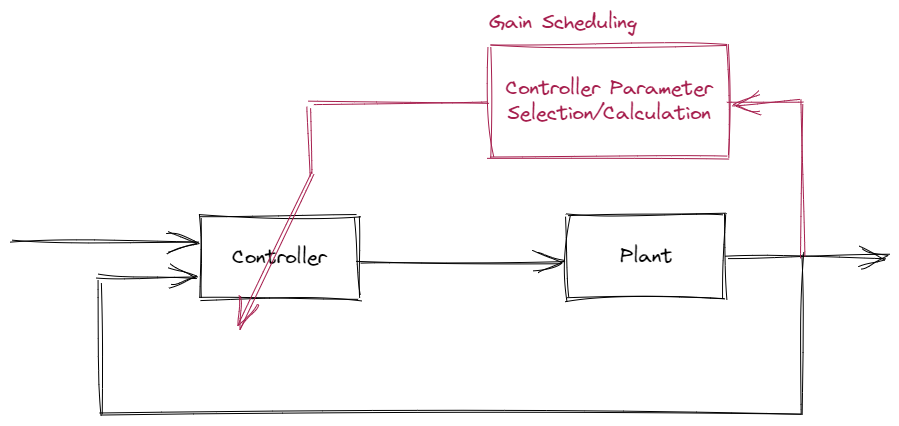
\includegraphics[width=300pt]{chapters/ch-adaptive-control-system/figures/gain_scheduling_schema.png}
	\caption{Gain scheduling schema.} \label{ch:acs:fig:gain_scheduling_schema}
\end{figure}

Gain scheduling is one of the most intuitive adaptive control schema, and has the earliest use case among all.

\vspace{0.1in}
\noindent \textbf{Model-Reference Adaptive System (MRAS)}
\vspace{0.1in}

In this scenario, a reference model is built that generates the “ideal” output of the closed-loop system given the reference point. This is often a virtual model that does not suffer from disturbances and error.

The MRAS then uses the output of both the actual plant and the reference model to calculate the controller parameter adjustment mechanism to minimize the difference between the outputs of the two models.

A demonstrative figure is given in Fig. \ref{ch:acs:fig:mars_schema}.

\begin{figure}
	\centering
	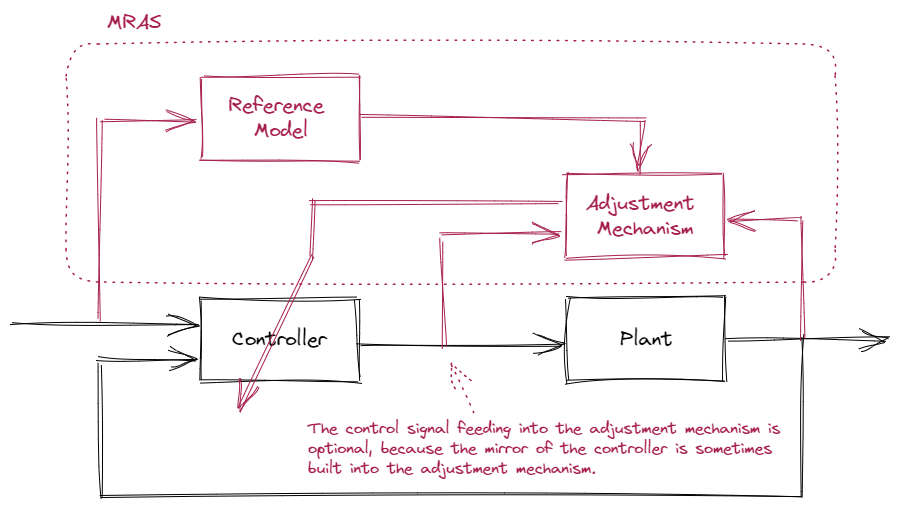
\includegraphics[width=300pt]{chapters/ch-adaptive-control-system/figures/mars_schema.png}
	\caption{MARS schema.} \label{ch:acs:fig:mars_schema}
\end{figure}

The MRAS is somewhat like a learning system. Usually, there is a “adaptation rate” (just like the learning rate) that controls the adapting speed.

\vspace{0.1in}
\noindent \textbf{Self-Tuning Regulator (STR)}
\vspace{0.1in}

The idea of STR is to estimate the system process and design and change the whole control system in real-time. Unlike the gain scheduling approach and MRAS where parameter adjustment mechanism is calculated in real-time, in STR approach, the controller designing problem is solved in real-time. From this sense, STR can be taken as the “high-end” gain scheduling problem.

A demonstrative figure is given in Fig. \ref{ch:acs:fig:str_schema}.

\begin{figure}
	\centering
	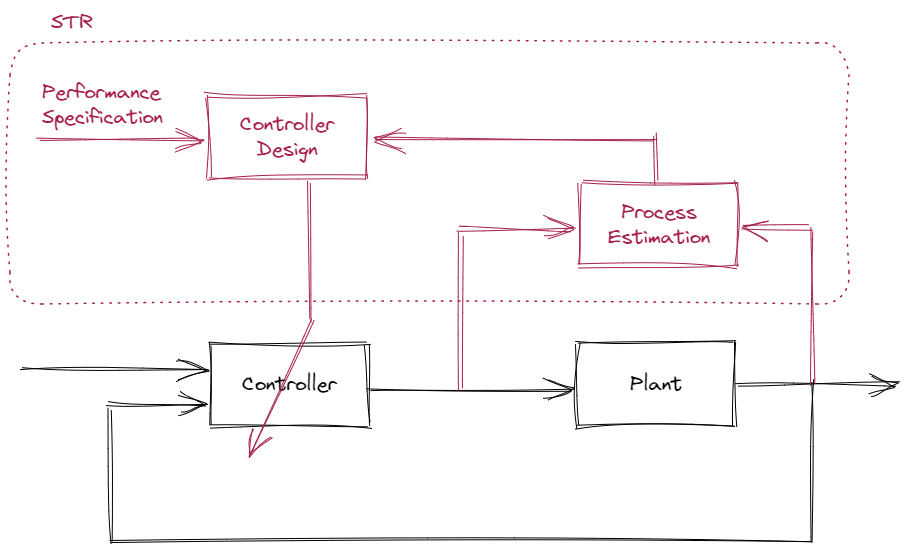
\includegraphics[width=300pt]{chapters/ch-adaptive-control-system/figures/str_schema.png}
	\caption{STR schema.} \label{ch:acs:fig:str_schema}
\end{figure}

STR can be made very flexible, because it is essentially a new control system design from scratch each time the environment changes.

\vspace{0.1in}
\noindent \textbf{Dual Control}
\vspace{0.1in}

The aforementioned adaptive control schemas do not taken into account the stochastics and statistics of the measurement and estimation uncertainty.

To analyze the performance of the system under estimation uncertainty and to develop control algorithm that can optimize the system performance under such uncertainty, nonlinear stochastic control theory needs to be used, which leads to the notion of dual control.

A demonstrative figure is given in Fig. \ref{ch:acs:fig:dual_schema}.

\begin{figure}
	\centering
	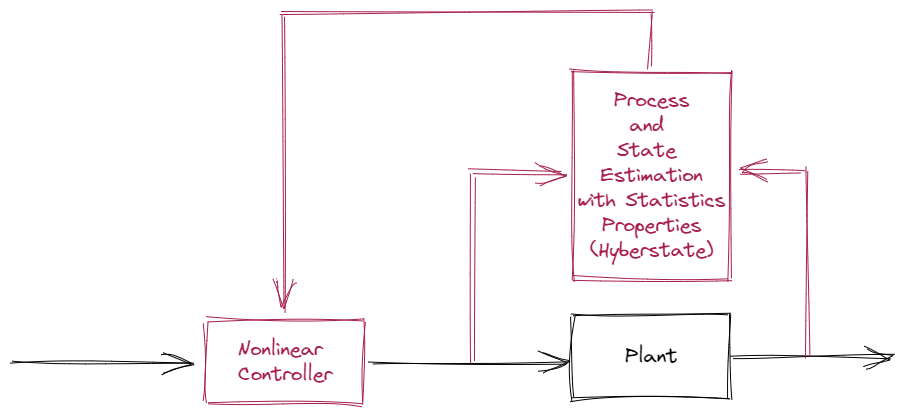
\includegraphics[width=300pt]{chapters/ch-adaptive-control-system/figures/dual_schema.png}
	\caption{Dual control schema.} \label{ch:acs:fig:dual_schema}
\end{figure}

This control system is essentially a nonlinear controller with a robust/adaptive filter that estimates the process dynamics and the states of the plant, together with statistics information of the estimates.

\subsection{A Typical Adaptive Control Problem Formulation}

For simplicity, consider the following LTI plant realizations.

Continuous time domain state space model:
\begin{eqnarray}
	\dot{x}(t) &=& Ax(t) + Bu(t) \nonumber \\
	y(t) &=& Cx(t) \nonumber
\end{eqnarray}

Continuous time domain transfer function model:
\begin{eqnarray}
	G(s) = \dfrac{B(s)}{A(s)} = \dfrac{b_0s^m + b_1s^{m-1} + \ldots + b_m}{s^n + a_1s^{n-1} + \ldots + a_n} \nonumber
\end{eqnarray}

Continuous time domain input-output model (with $p$ the differential operator, $p=\frac{d}{dt}$):
\begin{eqnarray}
	y(t) &=& G(p)u(t) \nonumber
\end{eqnarray}

Discrete time domain state-space model:
\begin{eqnarray}
	x(k+1) = Ax(k) + Bu(k) \nonumber \\
	y(k) = Cx(k) \nonumber
\end{eqnarray}

Discrete time domain transfer function:
\begin{eqnarray}
	G(z) = \dfrac{B(z)}{A(z)} = \dfrac{b_0z^m + b_qz^{m-1} + \ldots + b_m}{z^n + a_1z^{n-1} + \ldots + a_n} \nonumber
\end{eqnarray}

Discrete time domain input-output model (with $q$ the forward shift operator, $qy(t) = y(t+1)$):
\begin{eqnarray}
	y(k) &=& H(q)u(k) \nonumber
\end{eqnarray}

The above models may be describing the same plant, with different level of details. For example, when dealing with transfer function and input-output models, the initial condition of the system is often ignored. When dealing with discrete time domain plant model, it is open a sampled system derived from the original system.

If the parameters in the models are known, it is straight forward to design a closed-loop controller for them. This is called the underlying design problem. The adaptive control problem, on the other hand, is to design a controller without knowing the parameters. In response, the controller comes with adjustable control gains and associated adjustment mechanism.

A typical adaptive controller design shall include the following procedures:
\begin{enumerate}
	\item Characterize the desired closed-loop behavior.
	\item Determine a suitable control law with adjustable parameters.
	\item Design adjustment mechanism.
	\item Implement the control law with the parameters adjusted using the adjustment mechanism.
\end{enumerate}

Some successful use cases for adaptive control systems include
\begin{itemize}
	\item Automatic tuning controller, such as the PID automatic tuning controller. In practice, all conventional control systems can benefit from automatic parameter tuning, if done correctly.
	\item Gain scheduling, which is the standard technique used in flight control system for high-performance aircraft, and is becoming increasingly popular in industrial process control.
	\item Continuous adaptation control for continuously varying system.
	\item ``Human-in-the-loop'' control system.
\end{itemize}

Since adaptive control system is often more costly and complicated than a conventional constant-gain controller, it should be used wisely and not abused. If the dynamics of the system are manageable, consider using parametric model based control algorithm rather than the adaptive control system, the later of which is usually more complicated.

\section{Parameter Estimation}

Parameter estimation (or more generally, system identification) is widely used, either directly or indirectly, in many adaptive control schemas. An obvious example is STR, where the process dynamics estimation is built into the controller. Parameter estimation also happens implicitly in MRAS.

The key factors in system identification include the following.
\begin{itemize}
	\item Selection of model structure.
	\item Experiment design.
	\item Parameter and state estimation.
	\item Validation.
\end{itemize}

One thing to notice is that in adaptive control scope, the plant is assumed to change continuously, thus the parameter estimation needs to be done in a recursive manner.

\subsection{Least Squares Estimation}

Karl Friedrich Gauss defines LS estimation problem as follows.

\begin{VF}
\textbf{LS estimation:}
\\
\\
\noindent The parameters in the model should be chose such that the sum of the squares of the differences between the observed and the computed values, multiplied by numbers that measure the degree of precision, is a minimum.
\end{VF}

Notice that from the above definition, if all observations share the same degree of precision, the multipliers to all observations shall be the same, otherwise they should be different. Conventionally, the later case is referred as ``Weighted LS (WLS) estimation'' where each multiplier is called the ``weight'' associated with the observation. The more precise an observation, the higher its associated weight. On the other hand, the former case where all observations share the same precision is referred as LS estimation.

To reduce confusion, from now on LS estimation and WLS estimation are used to refer to the former and later cases, respectively.

Formulate LS estimation problem on a LTI system as follows. Let $\theta_i, i=1,...,n$ be $n$ unknown parameters in the model and $y(j), j=1,...,m$ be $m$ measurements collected from the mode. It is required that $m\geq n$. Variable $\phi_i(j)$ is called a regression variable (or a regressor) that links the measurements with the model parameters, so that
\begin{eqnarray}
	y(j) &=& \phi_1(j)\theta_1 + \phi_2(j)\theta_2 + \ldots + \phi_n(j)\theta_n + \epsilon(j) \label{eq:lsform1}
\end{eqnarray}
where $\epsilon(j)$ is assumed to be independent measurement noise associated with $y(j)$. Equation \eqref{eq:lsform1} is called a regression model. Putting \eqref{eq:lsform1} into matrix form gives
\begin{eqnarray}
	y &=& \Phi \theta + \epsilon \label{eq:lsform2}
\end{eqnarray}
where
\begin{eqnarray}
	y &=& \left[\begin{array}{ccc}
	              y(1) & \ldots & y(m)
	            \end{array}\right]^T \nonumber \\
	\Phi &=& \left[\begin{array}{ccc}
		\phi_1(1) & \ldots & \phi_n(1) \\
		\vdots & \ddots & \vdots \\
		\phi_1(m) & \ldots & \phi_n(m)
	\end{array}\right] \nonumber \\
	\theta &=& \left[\begin{array}{ccc}
	                   \theta_1 & \ldots & \theta_n
	                 \end{array}\right]^T \nonumber \\
    \epsilon &=& \left[\begin{array}{ccc}
                         \epsilon(1) & \ldots & \epsilon(m)
                       \end{array}\right]^T \nonumber
\end{eqnarray}
with $y$ the measurement vector, $\Phi$ the regression model matrix, and $\theta$ the unknown system parameter vector.

LS estimation of $\theta$ in \eqref{eq:lsform2} is formulated as follows. Select estimation $\hat{\theta} = [\hat{\theta}_1, ..., \hat{\theta}_n]^T$ so that the following cost function $V(\hat{\theta})$ is minimized.
\begin{eqnarray}
  V(\hat{\theta}) &=& \dfrac{1}{2}\sum_{i=1}^{m}e(i)^2 \label{eq:lscost}
\end{eqnarray}
where
\begin{eqnarray}
  e(i) &=& y(i) - \left(\phi_1(i)\hat{\theta}_1 + \phi_2(i)\hat{\theta}_2 + \ldots + \phi_n(i)\hat{\theta}_n\right) \nonumber \\
  &=& y(i) - \phi(i)^T\hat{\theta} \label{eq:lsmeasresidual2}
\end{eqnarray}
with
\begin{eqnarray}
  \phi(i)^T &=& \left[\begin{array}{ccc}
                        \phi_1(i) & \ldots & \phi_n(i)
                      \end{array}\right] \label{eq:lsmeasresidual3}
\end{eqnarray}
which is the $i$th row of $\Phi$. Variable $e(i)$ is called the residual.

Put everything into matrix format. Equation \eqref{eq:lscost} becomes
\begin{eqnarray}
	V(\hat{\theta}) &=& \dfrac{1}{2}\sum_{i=1}^{m} \left(y(i) - \phi(i)^T\hat{\theta}\right)^2 \nonumber \\
	&=& \dfrac{1}{2}(y - \Phi\hat{\theta})^T(y - \Phi\hat{\theta}) \label{eq:lsform3}
\end{eqnarray}
Denote $e = [e(1), ..., e(m)]^T$. From \eqref{eq:lsmeasresidual2},
\begin{eqnarray}
  e &=& y - \Phi\hat{\theta} \label{eq:lsmeasresidual1}
\end{eqnarray}
and \eqref{eq:lsform3} becomes
\begin{eqnarray}
	V(\hat{\theta}) &=& \dfrac{1}{2}e^Te \label{eq:lsform4}
\end{eqnarray}

The quadratic optimization problem given in \eqref{eq:lsform4} has the following unique analytical solution. Differentiating \eqref{eq:lsform4} w.r.t. $\theta$ gives (using numerator-layout notation)
\begin{eqnarray}
	\dfrac{dV(\hat{\theta})}{d\theta} &=& \dfrac{dV(\hat{\theta})}{de}\dfrac{de}{d\theta} \label{eq:lsform5} \\
	&=& -e^T\Phi \label{eq:lsform6}
\end{eqnarray}
Equating \eqref{eq:lsform6} to zero gives the minimum of \eqref{eq:lsform4} as follows.
\begin{eqnarray}
  -e^T\Phi &=& 0 \label{eq:lsform7}
\end{eqnarray}
Substituting \eqref{eq:lsmeasresidual1} into \eqref{eq:lsform7} gives
\begin{eqnarray}
- \left(y - \Phi\hat{\theta}\right)^T\Phi &=& 0 \nonumber \\
- \Phi^T\left(y - \Phi\hat{\theta}\right) &=& 0 \nonumber \\
 \Phi^T\Phi\hat{\theta} &=& \Phi^T y \nonumber \\
 \hat{\theta} &=& \left(\Phi^T\Phi\right)^{-1}\Phi^Ty \label{eq:lsform8}
\end{eqnarray}
provided that $\Phi^T\Phi$ is nonsingular, which is known as the excitation condition. Equation \eqref{eq:lsform8} is the solution to the LS estimation problem in \eqref{eq:lscost}.

\begin{mdframed}
\textbf{A Quick Note on Matrix Differentiation}
\\
\\
In numerator-layout notion, the scalar $V(\hat{\theta})$ differentiated w.r.t. the vector $e$ in \eqref{eq:lsform5} is given by
\begin{eqnarray}
	\dfrac{dV(\hat{\theta})}{de} &=& \left[\begin{array}{ccc}
		\dfrac{dV(\hat{\theta})}{de(1)} & \ldots & \dfrac{dV(\hat{\theta})}{de(m)}
	\end{array}\right] \nonumber \\
	&=& \left[\begin{array}{ccc}
		e(1) & \ldots & e(m)
	\end{array}\right] \nonumber \\
&=& e^T \nonumber
\end{eqnarray}

The vector $e$ differentiated w.r.t. the vector $\theta$ is given by
\begin{eqnarray}
\dfrac{de}{d\theta} &=& \left[\begin{array}{ccc}
                                \dfrac{de(1)}{d\theta_1} & \ldots & \dfrac{de(m)}{d\theta_n} \\
                                \vdots & \ddots & \vdots \\
                                \dfrac{de(m)}{d\theta_1} & \ldots & \dfrac{de(m)}{d\theta_n}
                              \end{array}\right] \nonumber \\
                              &=& \left[\begin{array}{ccc}
                                -\phi_1(1) & \ldots & -\phi_n(1) \\
                                \vdots & \ddots & \vdots \\
                                -\phi_1(m) & \ldots & -\phi_n(m)
                              \end{array}\right] \nonumber \\
                              &=& -\Phi \nonumber
\end{eqnarray}
where
\begin{eqnarray}
\dfrac{de(i)}{d\theta_j} &=& -\phi_j(i) \nonumber
\end{eqnarray}
because of \eqref{eq:lsmeasresidual2}.

Therefore,
\begin{eqnarray}
  \dfrac{dV(\hat{\theta})}{d\theta} = \dfrac{dV(\hat{\theta})}{de}\dfrac{de}{d\theta} = -e^T\Phi \nonumber
\end{eqnarray}
which is \eqref{eq:lsform6}.
\end{mdframed}

A WLS estimation problem can be formulated similarly, by changing \eqref{eq:lscost} with
\begin{eqnarray}
  V(\hat{\theta}) &=& \dfrac{1}{2}\sum_{i=1}^{m}w(i)e(i)^2 \nonumber
\end{eqnarray}

The solution to a WLS estimation can be similarly derived and the result is
\begin{eqnarray}
  \hat{\theta} &=& \left(\Phi^TW\Phi\right)^{-1}\Phi^TWy \nonumber
\end{eqnarray}
where $W = \textup{diag}(w(1), ...,w(m))$.

\subsection{Statistics Properties of LS Estimation}

In the discussions below, We will assume that all measurement noise $\epsilon(i), i=1,...,m$ are i.i.d. noise, whose mean and variance are zero and $\sigma^2$ respectively.

Substituting \eqref{eq:lsform2} into \eqref{eq:lsform8} gives
\begin{eqnarray}
  \hat{\theta} &=& \left(\Phi^T\Phi\right)^{-1}\Phi^T\left(\Phi\theta + \epsilon\right) \nonumber \\
  &=& \theta + \left(\Phi^T\Phi\right)^{-1}\Phi^T\epsilon \label{eq:lsform9}
\end{eqnarray}

Using \eqref{eq:lsform9}, the following statistics properties of LS estimation can be drawn.
\begin{eqnarray}
  E\left[\hat{\theta}\right] &=& \theta \nonumber \\
  \textup{Cov}\left[\hat{\theta}\right] &=& E\left[\hat{\theta}\hat{\theta}^T\right] \nonumber \\
  &=& \sigma^2\left(\Phi^T\Phi\right)^{-1} \nonumber
\end{eqnarray}
which suggests that the estimator is zero mean. With the fixed number $n$ of parameters to be estimated, the estimation variance decreases as the number $m$ of observations increases, and the variance converges to zero eventually. The variance of the noise $\sigma^2$ can potentially be estimated from the state estimate $\hat{\theta}$. Details are given as follows. Substituting \eqref{eq:lsform2}, \eqref{eq:lsform8} into \eqref{eq:lsmeasresidual1} gives
\begin{eqnarray}
  e &=& \left(I - \Phi\left(\Phi^T\Phi\right)^{-1}\Phi^T\right)\epsilon \label{eq:lsform10}
\end{eqnarray}
Using \eqref{eq:lsform10},
\begin{eqnarray}
  E\left[ee^T\right] &=& \sigma^2\left(I - \Phi\left(\Phi^T\Phi\right)^{-1}\Phi^T\right)\left(I - \Phi\left(\Phi^T\Phi\right)^{-1}\Phi^T\right)^T \label{eq:lsform11}
\end{eqnarray}
Taking the trace of matrix from both sides of \eqref{eq:lsform11} gives
\begin{eqnarray}
  E\left[e^Te\right] &=& (m-n)\sigma^2 \label{eq:lsform12}
\end{eqnarray}
From \eqref{eq:lsform4} and \eqref{eq:lsform12},
\begin{eqnarray}
  \sigma^2 &=& \dfrac{2}{m-n}E\left[V(\hat{\theta})\right] \nonumber
\end{eqnarray}
can be used to estimate the variance of the noise.

\subsection{Recursive LS Estimation}

Recursive state estimation allows ``updating'' the state estimate each time a new measurement set becomes available. It takes advantages of previously calculated state estimate with less measurements, instead of calculating everything from scratch, which is also known as the batch estimation. Recursive estimation saves computational and memory burden than the batch estimation. Given that observations are often naturally obtained sequentially in real time, recursive estimation has a large demand in practice.

Let each measurement be obtained associated with a incremental time stamp $k=1, 2, ...$. While the number of parameters to be estimated remains constant $n$, the number of measurement $m$ is dynamic and replaced by the notion $k$.

It is worth mentioning that the size of $\Phi$ in \eqref{eq:lsform2} grows with $k$, in the sense that each time a new measurement becomes available, $\Phi$ grows by one row. For convenience, $\Phi(k)$ is used to describe $\Phi$ in \eqref{eq:lsform2} when there are $k$ measurements.

As more and more measurements come in, the state estimate $\hat{\theta}$ also evolves and become more and more accurate. Denote $\hat{\theta}(k)$ the state estimate when up to $k$ measurements are available, $k \geq n$.

In recursive estimation schema, the estimator is formulated as a Markov process, and the state estimate $\hat{\theta}(k+1)$ is formulated as a function of $\hat{\theta}(k)$ and $y(k+1)$, and does not directly involve the earlier state estimates $\hat{\theta}(k-1), \hat{\theta}(k-2), ...$ or measurements $y(k), y(k-1), ...$. This is possible because the information of $\hat{\theta}(k-1), \hat{\theta}(k-2), ...$ and $y(k), y(k-1), ...$ are integrated into $\hat{\theta}(k)$.

The derivation of the recursive estimation is as follows. Notice that $\phi(i)^T$ in \eqref{eq:lsmeasresidual3} is the $i$th row of $\Phi(k)$, hence
\begin{eqnarray}
  \Phi(k)^T\Phi(k) &=& \sum_{i=1}^{k} \phi(i)\phi(i)^T \label{eq:recursivels1}
\end{eqnarray}
Assume that the excitation condition holds. Denote $P(k) = \left(\Phi(k)^T\Phi(k)\right)^{-1}$, or equivalently $P(k)^{-1} = \Phi(k)^T\Phi(k)$. Use \eqref{eq:recursivels1},
\begin{eqnarray}
  P(k+1)^{-1} &=& P(k)^{-1} + \phi(k+1)\phi(k+1)^T \label{eq:recursivels2}
\end{eqnarray}
which can be calculated recursively.

Rewrite \eqref{eq:lsform8} as follows.
\begin{eqnarray}
  \hat{\theta}(k) &=& \left(\sum_{i=1}^{k} \phi(i)\phi(i)^T\right)^{-1}\sum_{i=1}^{k}\phi(i)y(i) \nonumber \\
                  &=& P(k)\sum_{i=1}^{k}\phi(i)y(i) \nonumber \\
  \hat{\theta}(k+1) &=& \left(\sum_{i=1}^{k+1} \phi(i)\phi(i)^T\right)^{-1}\sum_{i=1}^{k+1}\phi(i)y(i) \nonumber \\
                    &=& P(k+1)\left(\sum_{i=1}^{k}\phi(i)y(i) + \phi(k+1)y(k+1)\right) \nonumber \\
                    &=& P(k+1)\left(P(k)^{-1}\hat{\theta}(k) + \phi(k+1)y(k+1)\right) \nonumber \\
                    &=& P(k+1)\left(\left(P(k+1)^{-1} - \phi(k+1)\phi(k+1)^T\right)\hat{\theta}(k) \right. \nonumber \\
                     && \left. + \phi(k+1)y(k+1)\right) \nonumber \\
                    &=& \hat{\theta}(k) \nonumber \\ && + P(k+1)\phi(k+1)\left(y(k+1) - \phi(k+1)^T\hat{\theta}(k)\right) \label{eq:recursivels3}
\end{eqnarray}

Equation \eqref{eq:recursivels2} and \eqref{eq:recursivels3} give the recursive LS estimation. Notice that the \eqref{eq:recursivels2} gives the recursive calculation of $P(k)^{-1}$. The recursive calculation of $P(k)$ can be easily derived from \eqref{eq:recursivels2} using matrix inversion lemma as follows.
\begin{eqnarray}
P(k+1) &=& P(k) - P(k)\phi(k+1) \nonumber \\ && \times \left(I + \phi(k+1)^TP(k)\phi(k+1)\right)^{-1}\phi(k+1)^TP(k) \nonumber \\
P(k+1)\phi(k+1) &=& P(k)\phi(k+1) \nonumber \\ && \times \left(I - \left(I + \phi(k+1)^TP(k)\phi(k+1)\right)^{-1}\right. \nonumber \\ &&  \left. \times \phi(k+1)^TP(k)\phi(k+1)\right) \nonumber \\
&=& P(k)\phi(k+1)\left(I + \phi(k+1)^TP(k)\phi(k+1)\right)^{-1} \nonumber \\ && \times \left(\left(I + \phi(k+1)^TP(k)\phi(k+1)\right) \right. \nonumber \\ && \left. - \phi(k+1)^TP(k)\phi(k+1)\right) \nonumber \\
&=& P(k)\phi(k+1)\left(I + \phi(k+1)^TP(k)\phi(k+1)\right)^{-1} \nonumber
\end{eqnarray}
where notice that in the above equations the identity matrix $I$ under the scope of our discussion should be $1$, as the measurement at any instant, $y(k)$, is a scalar. We followed the convention using $I$ because in practice, the measurement at any instant can be a vector. Hopefully this explanation helps to clear some confusion.

Denote $K(k) = P(k)\phi(k)$ the Kalman gain, and residual $\varepsilon(k+1) = y(k+1) - \phi(k+1)^T\hat{\theta}(x)$ the innovation vector, where $\phi(k+1)^T\hat{\theta}(x)$ can be interpreted as a ``guess'' of $y(k+1)$ using the state estimate $\hat{\theta}(x)$. Recursive LS estimation can be taken as a special case of Kalman filter where (a) measurement $y(k)$ is a scalar; (b) process matrix is unit matrix; (c) input and process noise are both zero.

\subsection{LS Estimation with Time-Varying Parameters}

If the parameter is time varying and has a solid dynamic model, considering using Kalman filter and other parametric model based estimators. If not, consider two scenarios: (a) parameters changes abruptly and infrequently; (b) parameters changes slowly and continuously.

Consider case (a). In this case, the abrupt changes can be detected from the magnitude of the innovation vector. The innovation vector covariance is jointly decided by the measurement noise and the state estimate precision. When the parameter is constant, the covariance matrix converges to a certain value that can be calculated analytically. A simple test can be used to detect when the innovation vector violates the statistics assumption, indicating that there is an abrupt parameters change.

In such case, just ``reset'' the system by assuming the new measurement is the first set of measurement collected by the system. In practice, this can be achieved equivalently by reset $P(k-1)$ and/or $P(k)$ to a diagonal matrix with large elements.

Consider case (b). One way to handle this parameter change is to use moving horizon estimation, or introducing a forgetting factor into the cost function. An example of introducing forgetting factor is given as follows. In \eqref{eq:lsform3}, set
\begin{eqnarray}
  V(\hat{\theta}) &=& \dfrac{1}{2}\sum_{i=1}^{k} \lambda^{k-i}\left(y(i) - \phi(i)^T\hat{\theta}\right)^2 \label{eq:recursivels4}
\end{eqnarray}
where $0 < \lambda < 1$ is a forgetting factor, and the method given in \eqref{eq:recursivels4} is called exponential forgetting. By introducing the forgetting factor, the contribution of innovation introduced by early measurements and state estimates to the cost function is reduced, thus reducing their impact on the state estimates.

The batch and recursive algorithms to calculate the state estimates for \eqref{eq:recursivels4} can be derived similarly. Some key derivations are given below.

Equation \eqref{eq:lsform8} becomes
\begin{eqnarray}
\hat{\theta} &=& \left(\Phi^T\Lambda\Phi\right)^{-1}\Phi^T\Lambda y \nonumber \\
\Lambda &=& \textup{diag}\left(\begin{array}{cccc}
                                 \lambda^{m-1} & \ldots & \lambda & 1
                               \end{array}\right) \nonumber
\end{eqnarray}

Equation \eqref{eq:recursivels2} becomes
\begin{eqnarray}
P(k)^{-1} &=& \Phi(k)^T\Lambda \Phi(k) \nonumber \\
P(k+1)^{-1} &=& \lambda P(k)^{-1} + \phi(k+1)\phi(k)^T \nonumber
\end{eqnarray}
Applying matrix inversion lemma to the above equation gives
\begin{eqnarray}
P(k+1) &=& \dfrac{1}{\lambda}P(k) - \dfrac{1}{\lambda}P(k)\phi(k+1) \nonumber \\ && \times \left(\lambda I + \phi(k+1)^TP(k)\phi(k+1)\right)^{-1}\phi(k+1)^TP(k) \nonumber \\
K(k+1) &=& P(k+1) \phi(k+1) \nonumber \\
&=&  P(k)\phi(k+1)\left(\lambda I + \phi(k+1)^TP(k)\phi(k+1)\right)^{-1} \nonumber
\end{eqnarray}

Equation \eqref{eq:recursivels3} has the same eventual form of
\begin{eqnarray}
  \hat{\theta}(k+1) &=& \hat{\theta}(k) + P(k+1)\phi(k+1)\left(y(k+1) - \phi(k+1)^T\hat{\theta}(x)\right) \nonumber
\end{eqnarray}

\subsection{Simplified LS Estimation: Projection Algorithm, SA, and LMS}

The recursive LS algorithm \eqref{eq:recursivels2} and \eqref{eq:recursivels3} requires the updates of $P(k)$ which involves matrix inversion, where $P(k)$ has a size of $n\times n$, and $n$ r2 the number of parameters to be estimated. When $n$ is large, this calculation can be time consuming.

Consider interpreting the cost function \eqref{eq:lsform3} as follows.
\begin{eqnarray}
    \hat{\theta}(k) &=& \arg \min_{\hat{\theta}} V_k(\hat{\theta})
    = \arg \min_{\hat{\theta}} \dfrac{1}{2}\sum_{i=1}^{k} \left(y(i) - \phi(i)^T\hat{\theta}\right)^2 \label{eq:projalgob} \\
    \hat{\theta}(k+1) &=& \arg \min_{\hat{\theta}} V_{k+1}(\hat{\theta})
    = \arg \min_{\hat{\theta}} \dfrac{1}{2}\sum_{i=1}^{k+1} \left(y(i) - \phi(i)^T\hat{\theta}\right)^2 \label{eq:projalgo1}
\end{eqnarray}
where
\begin{eqnarray}
  V_i(\hat{\theta}) &=& \dfrac{1}{2}\sum_{j=1}^{i} \left(y(j) - \phi(j)^T\hat{\theta}\right)^2 \nonumber
\end{eqnarray}
is the cost function formulated using the first $i$ measurements $y(1), ..., y(i)$.

Formulating \eqref{eq:projalgo1} as a function of $V_k(\hat{\theta})$ gives
\begin{eqnarray}
  \hat{\theta}(k+1) &=& \arg \min_{\hat{\theta}} \left[ V_k(\hat{\theta}) + \dfrac{1}{2} \left(y(k+1) - \phi(k+1)^T\hat{\theta}\right)^2\right] \label{eq:projalgo2}
\end{eqnarray}
We already know that $\hat{\theta}(k)$ minimizes $V_k(\hat{\theta})$ from \eqref{eq:projalgob}, and $V_k(\hat{\theta})$ happens to be the first term in \eqref{eq:projalgo2}. Therefore, \eqref{eq:projalgo2} is essentially an optimization problem that concerns the following terms
\begin{eqnarray}
  \lVert \hat{\theta} - \hat{\theta}(k) \rVert \label{eq:projalgo3}
\end{eqnarray}
and
\begin{eqnarray}
\lVert y(k+1) - \phi(k+1)^T\hat{\theta} \rVert \label{eq:projalgo4}
\end{eqnarray}
where $\lVert \cdot \rVert$ denotes the Euclidean norm of a vector, and the weights associated with the two terms in the optimization problem are determined by the covariance of the state estimate and measurement noise.

Consider a modification to the optimization problem in \eqref{eq:projalgo2} as follows. Let \eqref{eq:projalgo3} be the only term in the optimization, and \eqref{eq:projalgo4} be a equality constraint, i.e.,
\begin{eqnarray}
    \textup{min} && \dfrac{1}{2} \left(\hat{\theta} - \hat{\theta}(k)\right)^T\left(\hat{\theta} - \hat{\theta}(k)\right) \label{eq:projalgo5} \\
    \textup{s.t.} && y(k+1) - \phi(k+1)^T\hat{\theta} = 0 \label{eq:projalgo52}
\end{eqnarray}
Notice that this modified optimization problem given by \eqref{eq:projalgo5} does not necessarily give the same result as the original problem in \eqref{eq:projalgo2}. This is because $ \hat{\theta}(k+1)$ in \eqref{eq:projalgo2} may not meet the equality constraint. Nevertheless, \eqref{eq:projalgo5} is an approximation to $\hat{\theta}(k+1)$ in \eqref{eq:projalgo2}.

Optimization \eqref{eq:projalgo5} can be solved using Lagrange multiplier method. Details are neglected here, and the result is given by
\begin{eqnarray}
  \hat{\theta}(k+1) &=& \hat{\theta}(k) + \dfrac{\phi(k+1)}{\phi(k+1)^T\phi(k+1)}\left(y(k+1) - \phi(k+1)^T\hat{\theta}(k)\right) \nonumber \\ && \label{eq:projalgo6}
\end{eqnarray}

Parameters $0 < \gamma < 2$ and $\alpha > 0$ are added to \eqref{eq:projalgo6} as shown below. The motivations of adding $\gamma$ and $\alpha$ are to make it possible to change the step length of the parameter adjustment and to avoid a potential problem what would occur when $\phi(k+1)=0$.
\begin{eqnarray}
  \hat{\theta}(k+1) &=& \hat{\theta}(k) + \dfrac{\gamma\phi(k+1)}{\alpha + \phi(k+1)^T\phi(k+1)}\left(y(k+1) - \phi(k+1)^T\hat{\theta}(k)\right) \nonumber \\ && \label{eq:projalgo7}
\end{eqnarray}
which is known as the projection algorithm. The choice $0 < \gamma < 2$ guarantees the convergency of \eqref{eq:projalgo7}.

One may think the quality constraint \eqref{eq:projalgo52} is too strong. When measurement error is considered, a modified version of \eqref{eq:projalgo6} is given below.
\begin{eqnarray}
\hat{\theta}(k+1) &=& \hat{\theta}(k) + \dfrac{\phi(k+1)}{\sum_{i=1}^{k+1}\phi(i)^T\phi(i)}\left(y(k+1) - \phi(k+1)^T\hat{\theta}(k)\right) \nonumber \\ && \label{eq:projalgo8}
\end{eqnarray}
which is known as the stochastic approximation (SA) algorithm.

A further simplification to \eqref{eq:projalgo7} and \eqref{eq:projalgo8} is given below.
\begin{eqnarray}
\hat{\theta}(k+1) &=& \hat{\theta}(k) + \gamma\phi(k+1)\left(y(k+1) - \phi(k+1)^T\hat{\theta}(k)\right) \nonumber
\end{eqnarray}
which is known as the least mean square (LMS) algorithm.

\subsection{Models}

The LS estimation algorithm can be applied to the models introduced in this section. By assuming a model, experiments can be designed and empirical data can be collected which serves as the input to the LS estimation algorithm. The parameters of the model can then be decided.

The initial states of the plant is ignored for now. In practice, with the model and parameters known, state estimation is carried out to determine the state of the system.

\vspace{0.1in}
\noindent \textbf{Finite Impulse Response (FIR) Model}
\vspace{0.1in}

An LTI system can be uniquely characterized by its impulse response. A demonstrative figure is given in Fig. \ref{ch:acs:fig:impulse_second_demo}. For an asymptotically stable system, the transient will converge to zero exponentially fast, depending on the position of the poles in the transfer function.
\begin{figure}
	\centering
	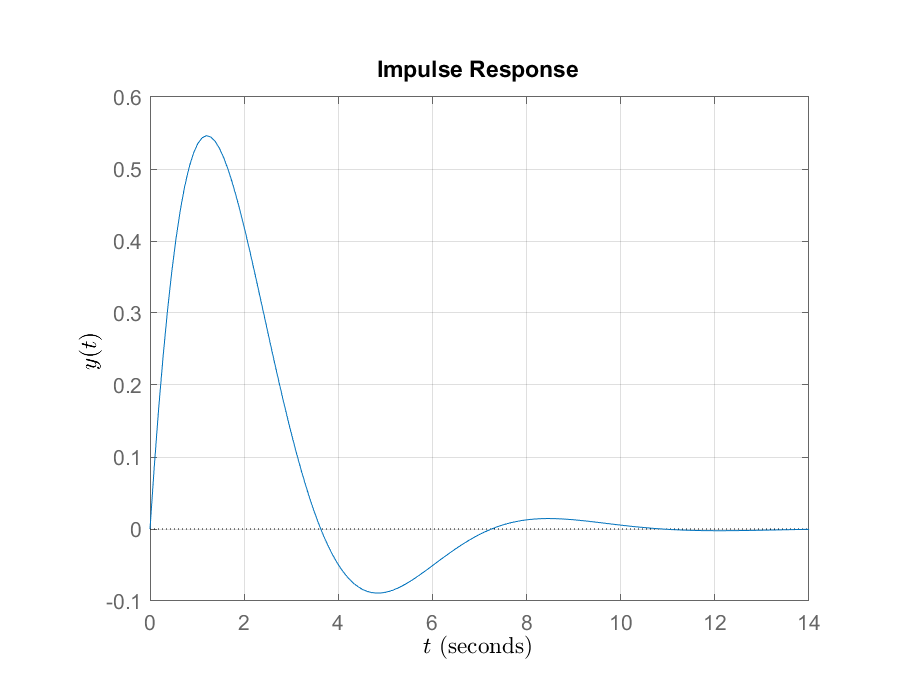
\includegraphics[width=350pt]{chapters/ch-adaptive-control-system/figures/impulse_second_demo.eps}
	\caption{LTI system impulse response demonstration.} \label{ch:acs:fig:impulse_second_demo}
\end{figure}

Consider sampling the outputs of Fig. \ref{ch:acs:fig:impulse_second_demo} in discrete time domain. The input at $k$, i.e., $u(k)$, would affect the consequent outputs $y(k+1), y(k+2), ...$. This sequence can go infinitely long in theory, but in practice we only consider the first finite number of outputs before $y$ settles to zero. The length of the sequence is determined by the sampling period and the time constant of the system.

Due to the superposition of the LTI system, the above also indicates that output of the system at $k$, i.e., $y(k)$, is affected by the past input signals $u(k-1), u(k-2), ...$, as given by the following equation. Likewise, only finite number of inputs are included in the equation.
\begin{eqnarray}
	y(k) &=& b_1u(k-1) + b_2u(k-2) + \ldots + b_nu(k-n) \label{eq:firmodel}
\end{eqnarray}

Equation \eqref{eq:firmodel} is known as the FIR model of a system. It has $n$ parameters to be estimated, and it fits well into the LS estimation schema described by \eqref{eq:lsform1}.

















